\documentclass[11pt,letterpaper]{article}
\usepackage[utf8]{inputenc}
\usepackage{amsmath}
\usepackage{amsfonts}
\usepackage{indentfirst}
\usepackage{graphicx}
\usepackage{setspace}
\usepackage[letterpaper,bindingoffset=0.2in,%
            left=1.5in,right=1in,top=1in,bottom=1in,%
            footskip=.25in]{geometry}
\author{Chathun Kurera}
\title{Dual Booting Windows 7 x64 and Ubuntu 14.04LTS in UEFI}
\begin{document}

\onehalfspacing

\section{Introduction}
The main purpose of this report is to document the  

\section{SSD Trim Support}
% {http://solid-state-drive-review.toptenreviews.com/what-is-trim-support.html}

Two types of storage devices that can be used in everyday desktop/laptop computers are HDD(Hard Disk Drive) and SSD(Solid State Drive). In a hard disk drive, data is written to one or more platters using a magnetic head 


The storage device used to install both Windows 7 and Ubuntu 14.04 in this report is a SSD(solid state drive). 


\begin{quote}
Imagine, if you will, that you have a stack of blank papers on your desk at work. Each workday you keep the papers with important information on them, but get rid of the unnecessary papers, like the one you doodled on during a boring meeting, by putting them in the "To Be Recycled" tray on your desk. It's not worth going all the way down to the recycling center for a few sheets of paper, so you wait until you have a stack that is worth the travel time.

Eventually, you run out of blank paper. Since you have a project due that day, it is now time to use the paper from the "To Be Recycled" tray. You take out your eraser and get to work. Erasing takes a lot of effort, so you decide to only clean up a portion of the stack to tide you over for a while. Eventually you will run out of paper again and you'll have to erase another portion, but you plan on crossing that bridge when you come to it. 
\end{quote}


\section{Setting up the UEFI}
UEFI(Unified Extensive Firmware Interface)replaces the traditional BIOS(Basic Input/Output System) that has been used to boot PCs since 1975. Manufactures started using a UEFI in the late 2010 instead of a BIOS due to its many advantages and with the release of Windows 8, Microsoft has pushed vendors to use UEFI only booting processes.


UEFI should be configured to the optimal settings before installing Windows 7.
	\subsection{Upgrade UEFI version}
	Older versions of UEFI lacks to support many features including dual booting of operating systems. Therefore, it is recommended to always check for an update before installing an operating system.
	
	\begin{figure}[]
      \centering
      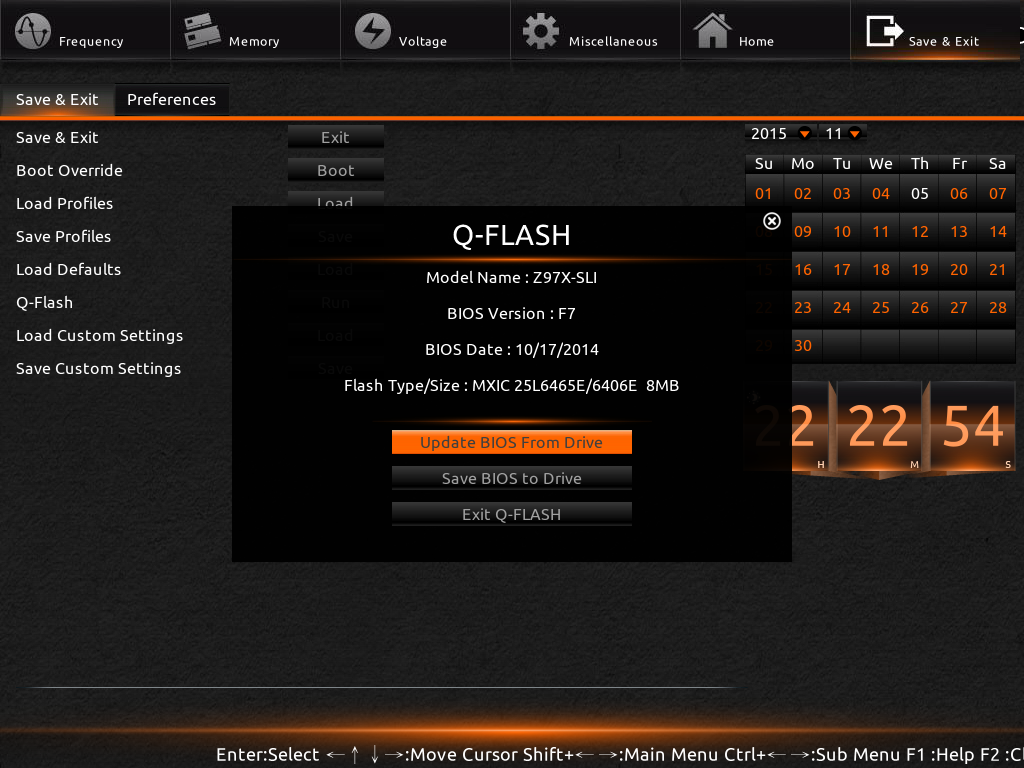
\includegraphics[width=0.8\textwidth]{q-flash}
      \caption{Flash UEFI BIOS}
      \label{fig:Flash_UEFI_BIOS}
    \end{figure}
	
	\subsection{Storage Configuration}
	The storage configuration should be set to AHCI(Advance Host Controller Interface).
	\subsection{Disable Secure Boot}
	Secure boot is feature that is enabled in UEFI that does not allow unauthorized operating systems and software from booting during the startup process. There exists a Microsoft signature in Windows 8 64 Bit and newer systems that the secure boot will accept. Therefore, secure boot needs to be disabled for a Windows 7 64 Bit installation. 
	\subsection{CSM}
	CSM(Compatibility Support Module) should be enabled and set to UEFI only so that Windows 7 and Ubuntu will not be installed in legacy mode.
	

\section{Installing Windows 7}
	\subsection{Offset partition alignment}

\section{Installing Ubuntu}



\section{Conclusions}

\singlespacing

\section*{Glossary}

\section*{References}

\end{document}